\chapter{Analiza otrzymanych wyników}
\label{cha:analiza_otrzymanych_wynikow}


\section{Analiza działania użytych algorytmów}

W celu implementacji algorytmu wyszukania optymalnych tras, w aplikacji została zaimplementowana obsługa kilku algorytmów wyszukiwania ścieżek w grafie. Standardowo aplikacja korzysta tylko z jednego z nich, implementacja ma na celu tylko ich porównanie. W poniższych akapitach przedstawiono testy porównawcze prędkości działania algorytmów podczas wyznaczania tras pomiędzy zestawem wybranych losowo punktów na mapie Krakowa. 
W celu heterogenizacji wyznaczonych tras, punkty początkowe i końcowe każdej z nich zostały dobrane w taki sposób, aby pokryły odpowiedni obszar Krakowa, a także przebiegały w miejscach, gdzie znajduje się zarówno dużo, jak i mało ścieżek zawartych w posiadanym zbiorze danych. Z tego powodu niektóre z nich przebiegają w okolicach rynku, a inne przez Wolę Justowską, gdzie jedyną ścieżką w posiadanym zbiorze jest droga po wale rzeki Rudawy.
Obydwa z zaimplementowanych algorytmów gwarantują każdorazowo wyznaczenie optymalnej trasy. Nie kończą one przeszukiwania po uzyskaniu pierwszej znalezionej trasy, stąd porównanie można uznać za miarodajny wynik złożoności obliczeniowej każdego z algorytmów.

\subsection{Porównanie działania algorytmu z wykorzystaniem algorytmu Dijkstra i A*}

Na poniższym wykresie zestawiono czasy działania obydwu algorytmów wraz z opisem trasy, dla której każdy z czasów został wyznaczony.

\begin{figure}[H]
\centering
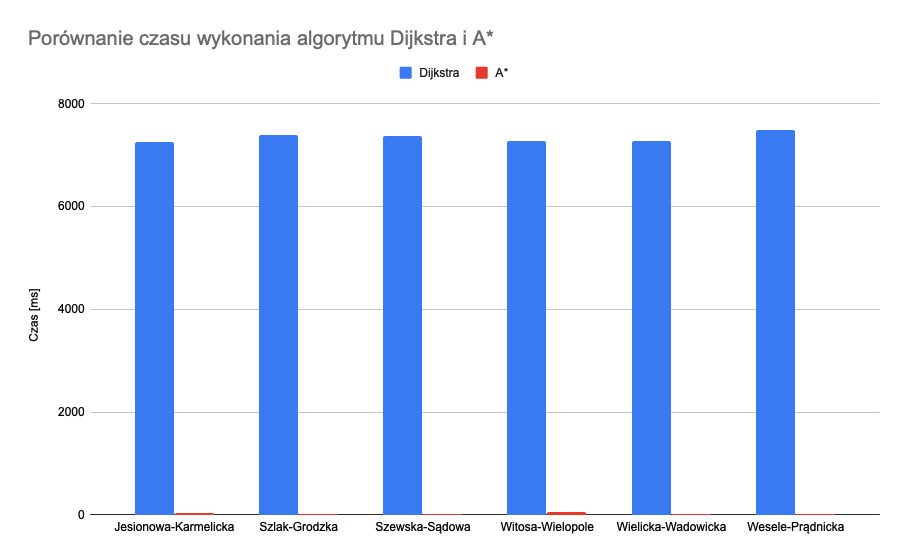
\includegraphics[width=0.7\textwidth]{czas_dijkstra_vs_a}
\caption{Czasy wykonania algorytmu Dijkstra i A* dla wybranych danych testowych.}
\end{figure}

Z wykresu można odczytać, że algorytm A* sprawdza się nieporównywalnie lepiej w stosunku do algorytmu Dijkstra w kontekście czasu wykonania. Z wykresu niełatwo jest nawet odczytać różnice w czasie działania ze względu na minimalny wkład czasów osiągniętych przez A*. W najgorszym z zaprezentowanych przypadków jego działanie było około 200-krotnie szybsze, zaś w najlepszym z przypadków różnica w prędkości działania była prawie 500-krotna. Z powyższego zestawienia jasno wynika, że do produkcyjnego zastosowania w aplikacji, w porównaniu z algorytmem Dijkstra, nadaje się tylko algorytm A*. Jest on za to znacznie bardziej czasochłonny w implementacji, stąd jego zastosowanie do zdecydowanie mniej złożonych grafów może być korzystniejsze. W celu zminimalizowania czasu wykonywania algorytmu Dijkstra można było zastosować odpowiednie zmniejszenie grafu na podstawie filtracji wierzchołków, które znajdują się wewnątrz obszaru na mapie zawartego przez punkt końcowy i początkowy. Jednak ze względu na brak potrzeby optymalizacji i odpowiednią wizualizację różnic czasu działania zaniechano tej modyfikacji.
W przypadku przeszukiwania grafu, w którym wierzchołki mogą być określone jako punkty na mapie, algorytm A* jest zdecydowanie szybszy ze względu na prostotę wyznaczenia heurystyki. W tym wypadku przewidywanie czy droga zbliża się do końca może być określone przez wyznaczenie odległości pomiędzy kolejnym sprawdzanym wierzchołkiem a punktem końcowym trasy. Dzięki temu, w przeciwieństwie do algorytmu Dijkstra, A* nie prowadzi przeszukania całego grafu przed wyznaczeniem optymalnej ścieżki, a ogranicza się jedynie do przeszukania szeregu dróg które prowadzą pomiędzy punktem końcowym i początkowym. \newline

Ogólną złożoność obliczeniową algorytmu A* przedstawiono poniższym wzorem.

// tutaj wzór na złożoność ogólną A*

Dla przykładu algorytmu użytego w aplikacji może zostać wyznaczona wzorem:

// tutaj wzór na złożoność A* w tym przypadku.

Na podstawie wzoru widać, że złożoność algorytmu A* w dużej mierze zależy od złożoności obliczeniowej wyznaczenia heurystyki. W przypadku, gdy proces ten przedstawiałby się złożonością obliczeniową O(n2), algorytm działałby z prędkością porównywalną do algorytmu Dijkstra.

\subsection{Czas działania algorytmu A* i Dijkstra w zależności od długości trasy}

Na poniższych wykresach przedstawiono czas działania algorytmu A* i Dijkstra w zależności od obszaru objętego przeszukiwaniem. W tym celu, na terenie Krakowa, wyznaczono zestaw tras w zakresie od bardzo krótkich, obejmujących tylko kilkaset metrów, do takich, które obejmują teren całego Krakowa.

\begin{figure}[H]
\centering
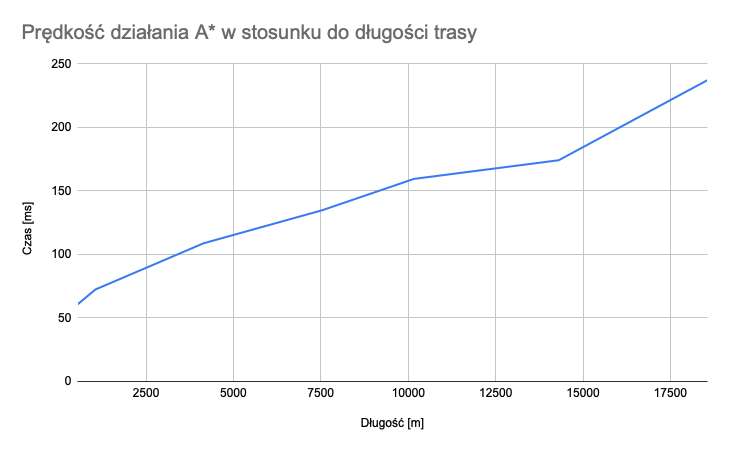
\includegraphics[width=0.7\textwidth]{a_a_dlugosc_trasy}
\caption{Czas wykonywania algorytmu A* w zależności od długości wyznaczonej trasy.}
\end{figure}

\begin{figure}[H]
\centering
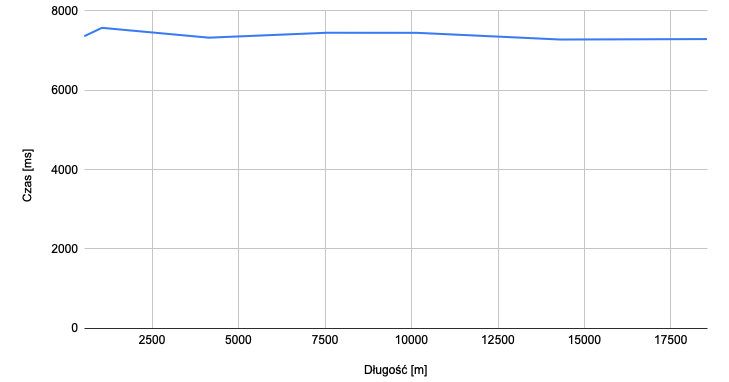
\includegraphics[width=0.7\textwidth]{dijkstra_a_dlugosc_trasy}
\caption{Czas wykonywania algorytmu Dijkstra w zależności od długości wyznaczonej trasy.}
\end{figure}

Z przedstawionych wykresów można odczytać, że czas działania algorytmu Dijkstra nie zależy od długości wyznaczonych tras. Delikatne fluktuacje czasu wykonania zależą od aktualnego użycia pamięci i procesora komputera podczas wykonywania testu. Jest to spowodowane zasadą działania algorytmu Dijkstra, który w każdym przypadku w pierwszej kolejności wykonuje obliczenia najkrótszych ścieżek pomiędzy wszystkimi wierzchołkami grafu.
Przeciwny przypadek obowiązuje dla algorytmu A*, który dzięki zastosowaniu heurystyki jest w stanie wykryć, gdy najkrótsza ścieżka została już odnaleziona i zatrzymać przeszukiwanie w odpowiednim przypadku. Z tego powodu w zależności od obszaru grafu obejmowanego przez przeszukanie, algorytm A* wykazuje znaczny, liniowy wzrost czasu wykonania.

\subsection{Porównanie algorytmu zachłannego A* i standardowej implementacji A*}

Kolejnym etapem analizy jest określenie czasu oraz jakości działania algorytmu zachłannego A* w stosunku do podstawowej wersji A*. W przeciwieństwie do standardowej implementacji, algorytm zachłanny, zyskując na czasie wykonania, nie gwarantuje wyznaczenia optymalnej ścieżki pomiędzy wierzchołkiem początkowym i końcowym. Bazując na przekazanej heurystyce, stara się wyznaczyć najlepsze lokalne rozwiązania podzbiorów składających się na wynikową trasę, następnie łączy uzyskane podzbiory w celu wyznaczenia trasy. W poniższych akapitach zawarto analizę czasu wykonania oraz wyznaczonych wag tras w zależności od typu algorytmu.

Na poniższym wykresie przedstawiono zestawienie wag tras wyznaczonych przez obydwa algorytmy dla uprzednio wyznaczonego zestawu dróg testowych.

\begin{figure}[H]
\centering
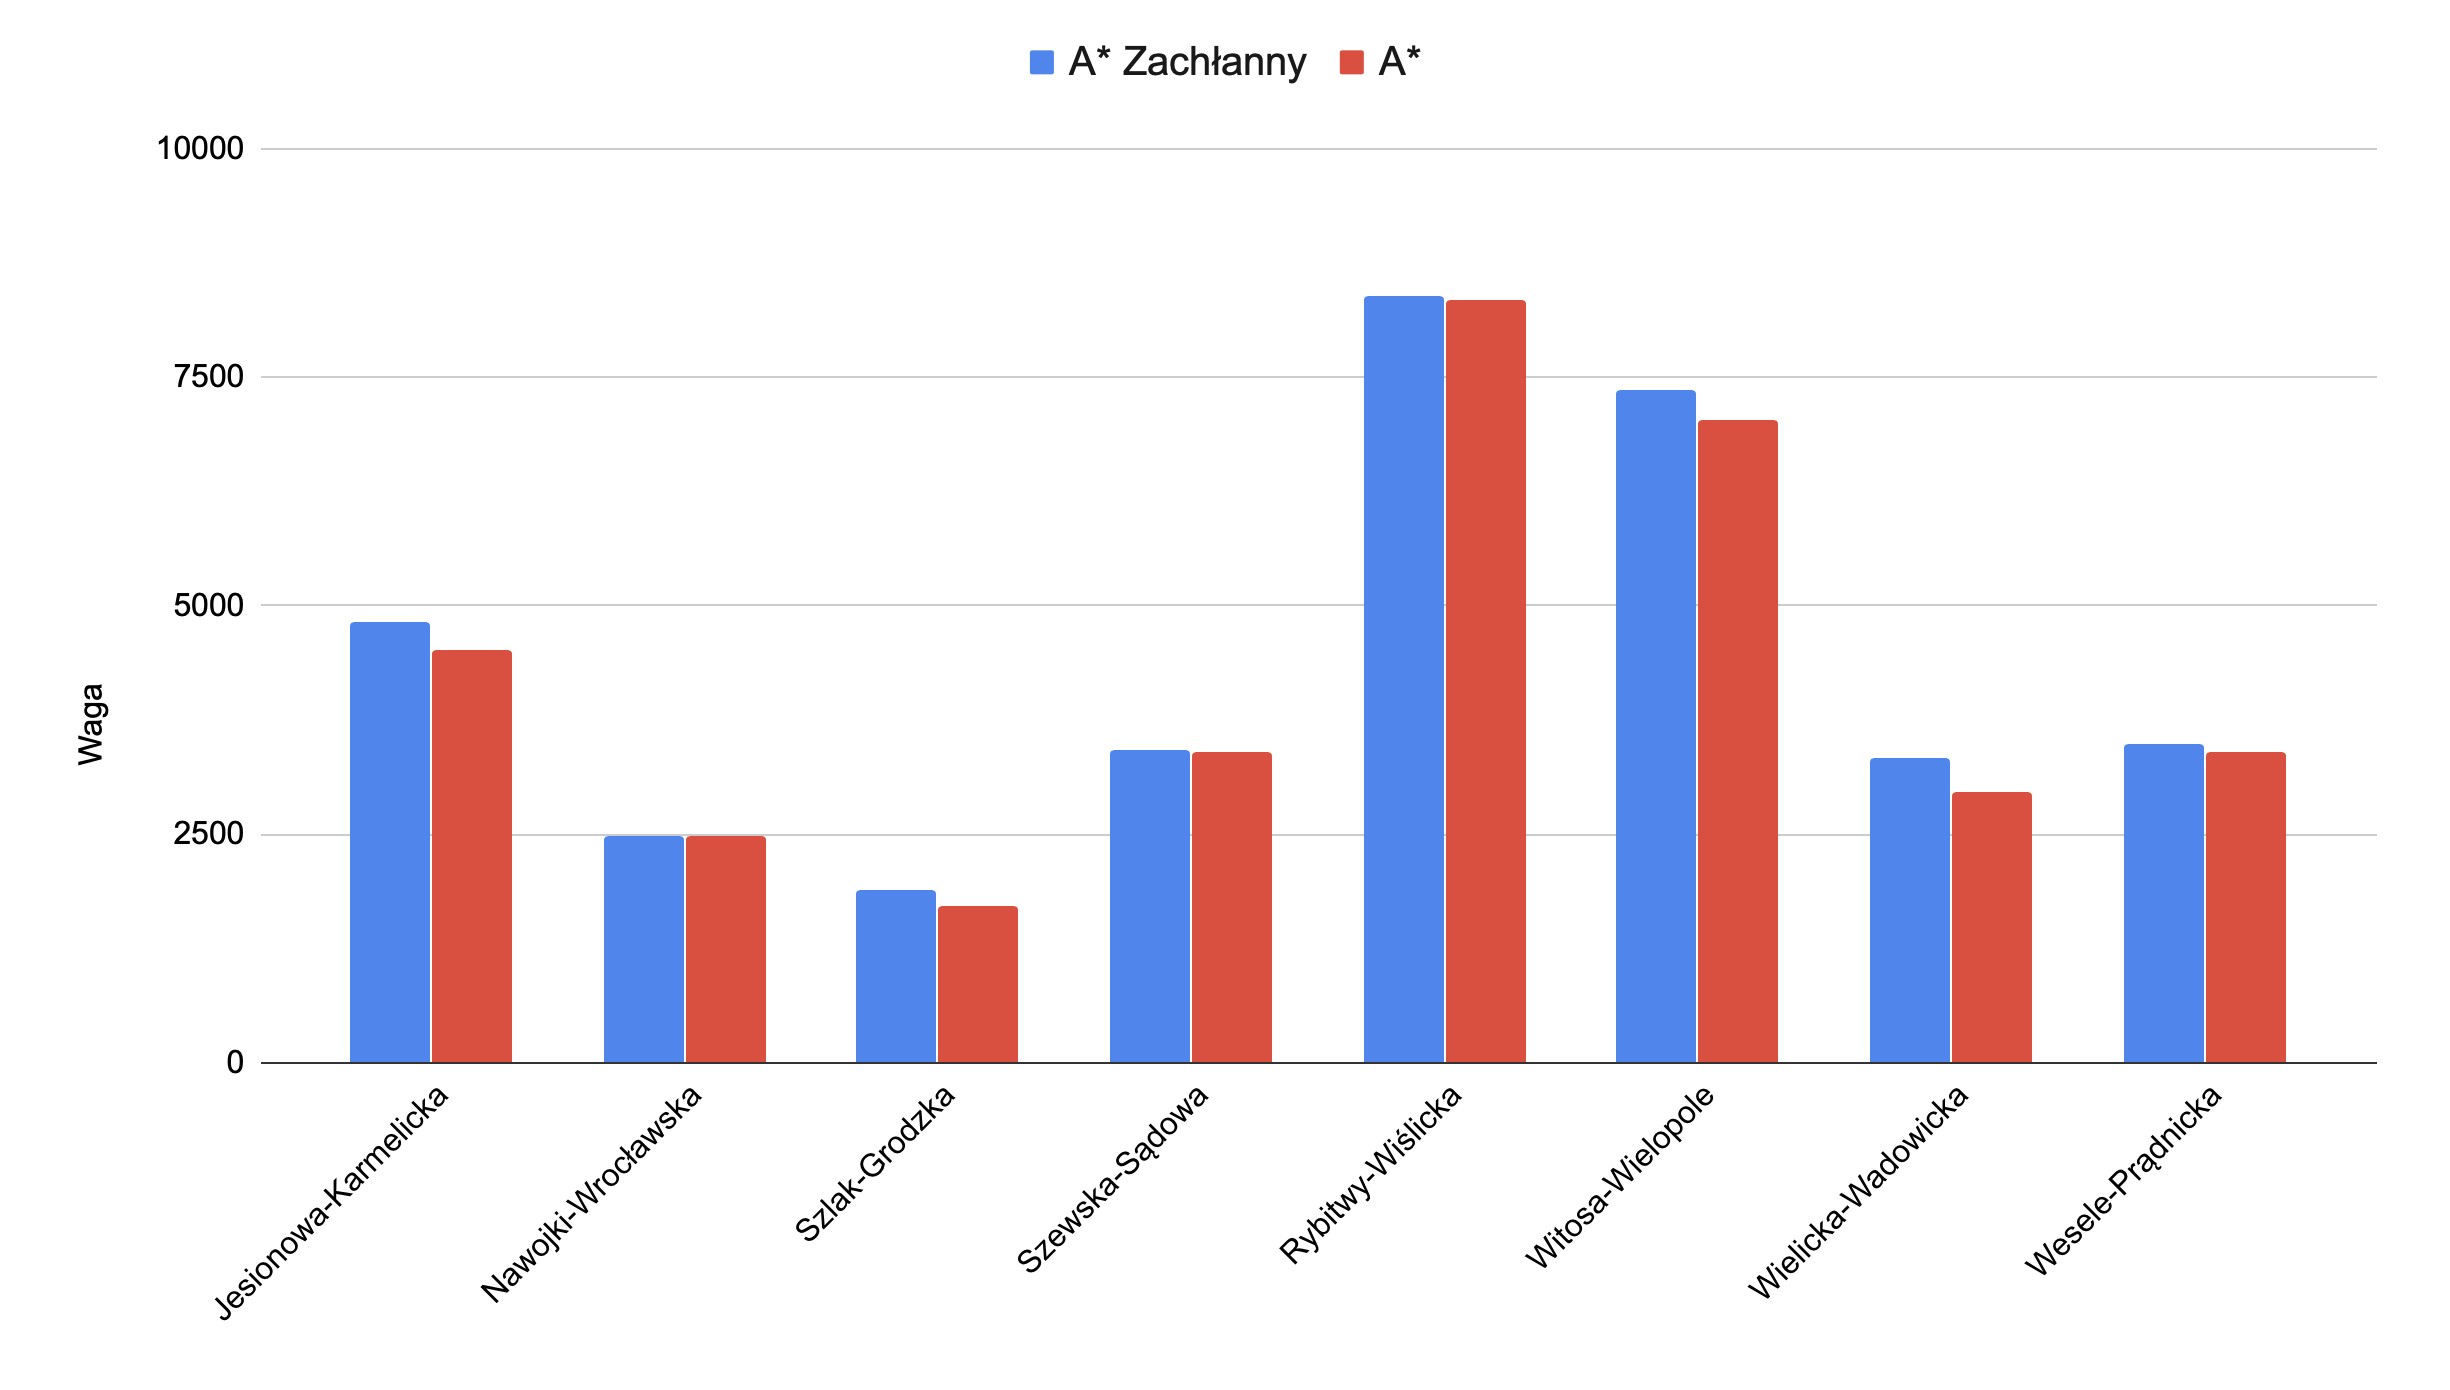
\includegraphics[width=0.7\textwidth]{waga_a_vs_a_greedy}
\caption{Zestawienie wag wyznaczonych przez algorytm A* oraz A* zachłanny dla wybranego zestawu danych testowych.}
\end{figure}

Korzystając z wartości przedstawionych na powyższym wykresie można odczytać, że poza przypadkiem bardzo krótkiej drogi pomiędzy ulicami Nawojki i Wrocławską, zachłanna odmiana algorytmu A* w każdym wypadku wyznaczyła trasę, która z punktu widzenia wagi jest gorsza niż ta wyznaczona przez standardową odmianę algorytmu A*.

Na poniższym wykresie przedstawiono zestawienie czasu działania dla uprzednio wyznaczonego zestawu testowych ścieżek.

\begin{figure}[H]
\centering
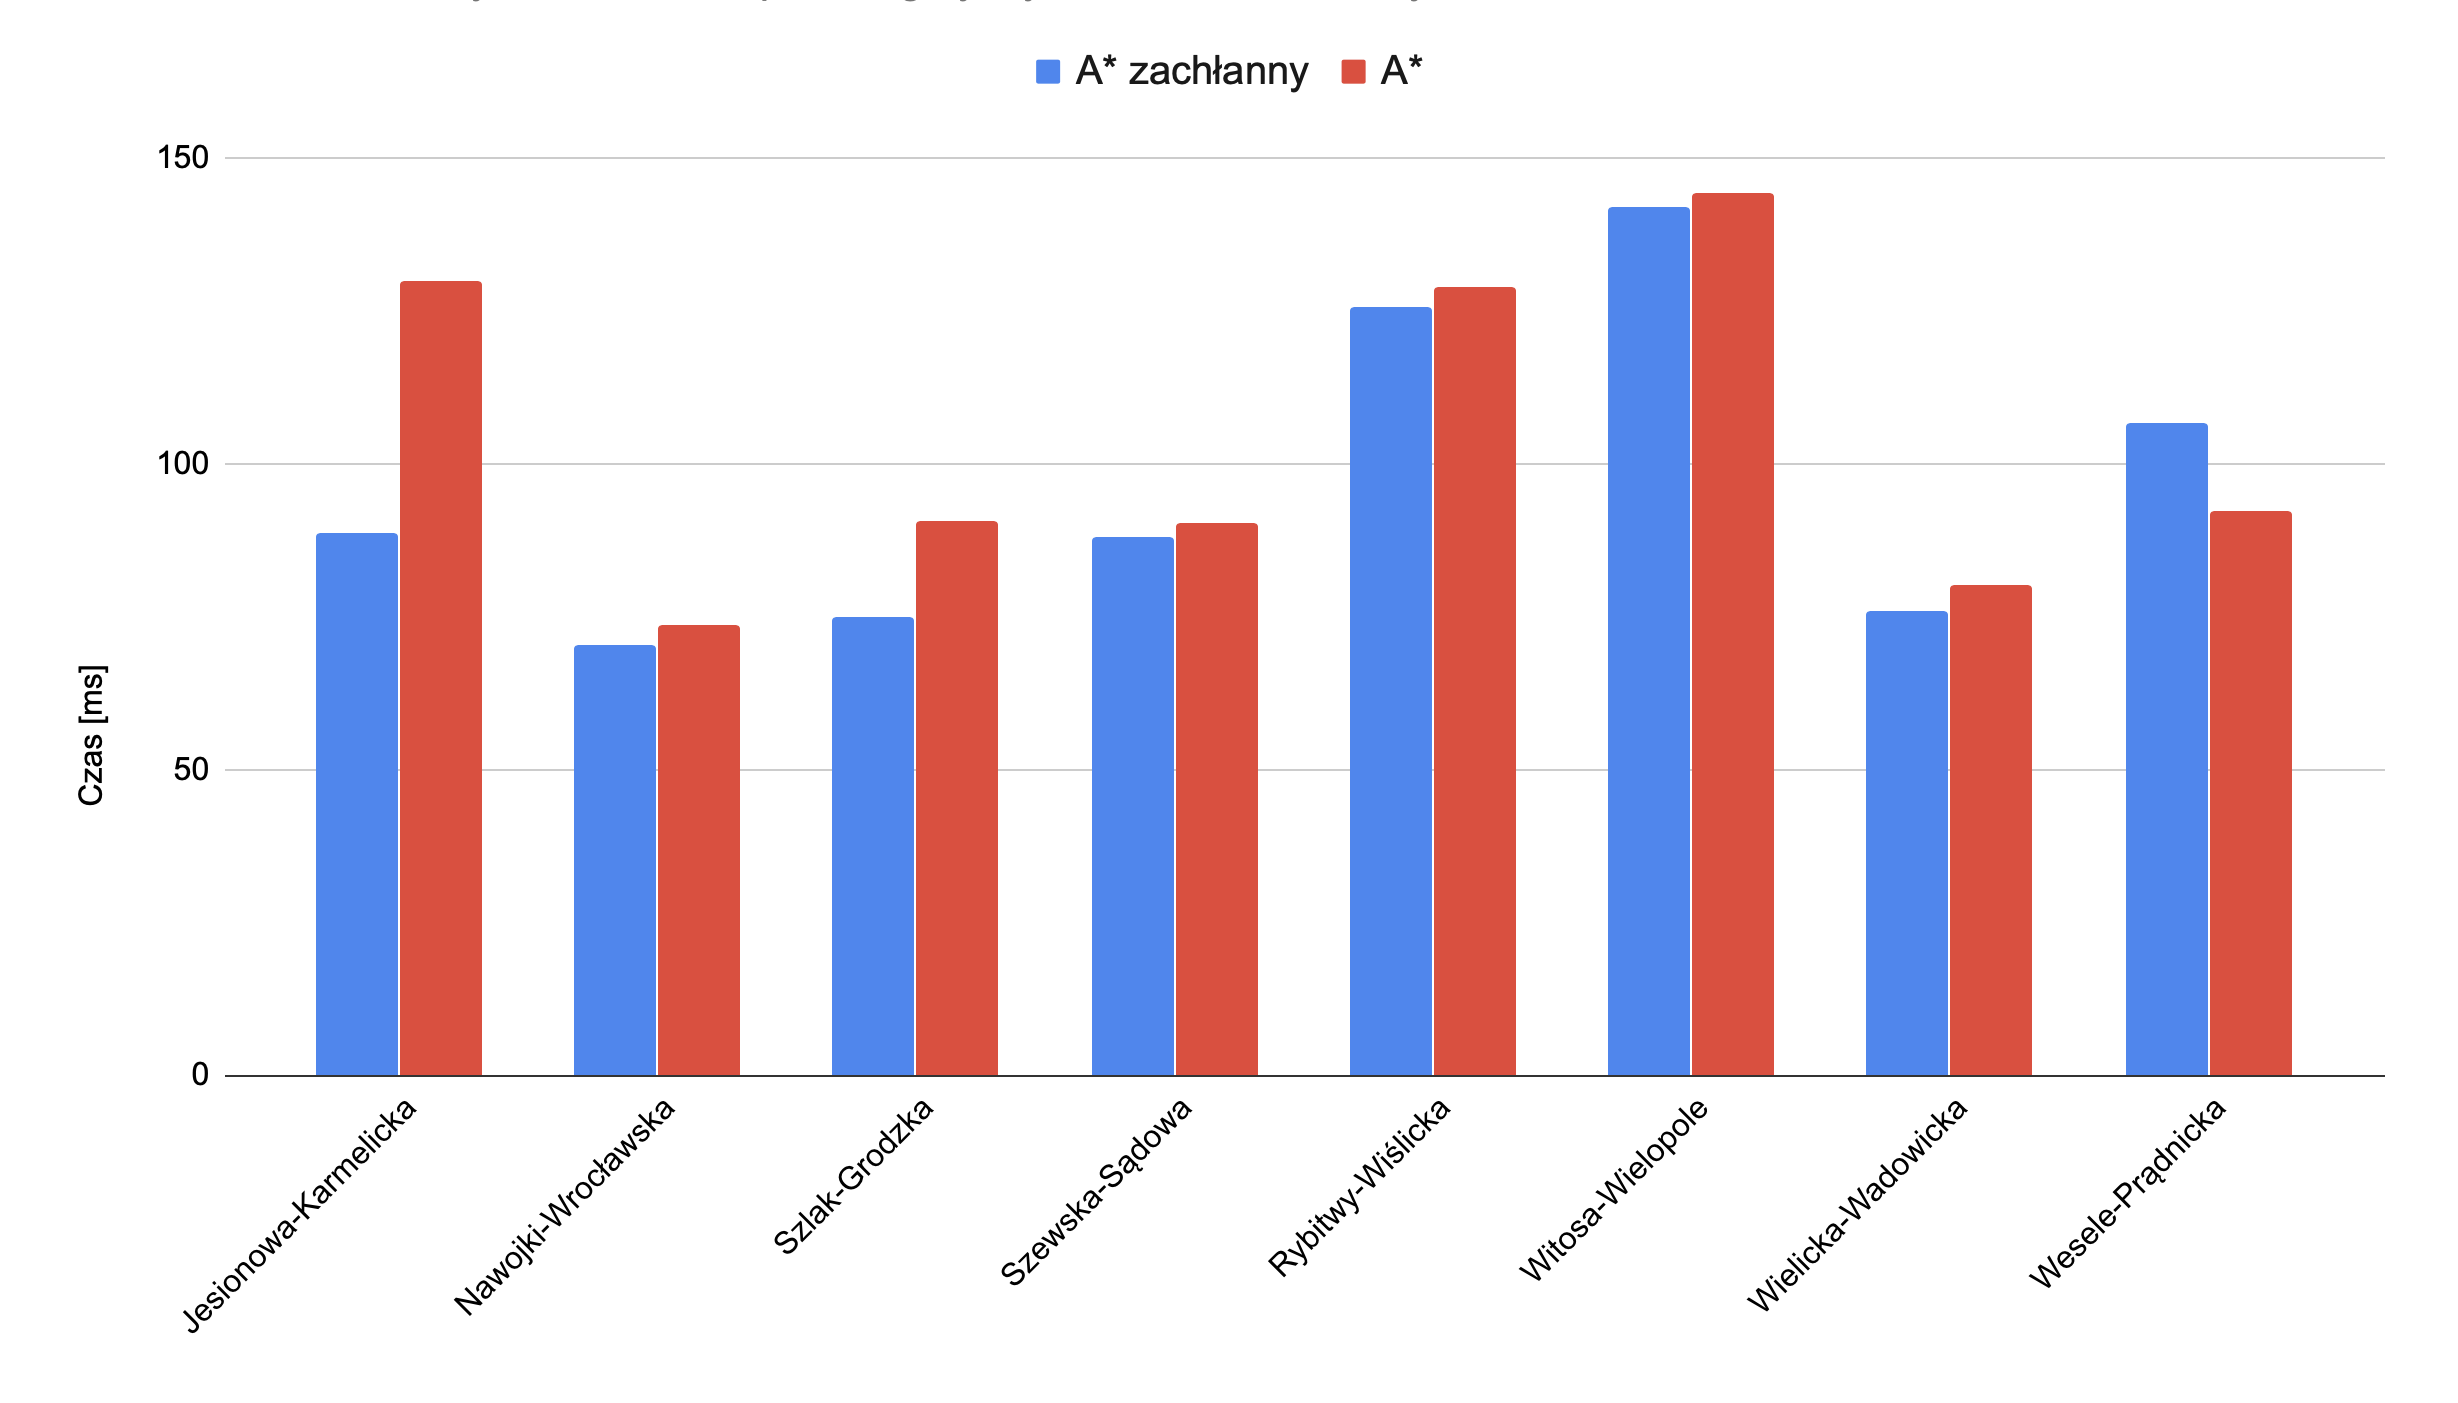
\includegraphics[width=0.7\textwidth]{czas_a_vs_a_greedy}
\caption{Zestawienie czasów wykonania algorytmów A* oraz A* zachłannego dla wybranego zestawu danych testowych.}
\end{figure}

Za wyjątkiem jednego przypadku, który może być spowodowany chwilową mniejszą wydajnością maszyny na której działały testy, algorytm zachłanny uzyskał lepszy średni czas wyznaczania trasy. Jest to spodziewany rezultat, ponieważ algorytm ten w swojej zasadzie działania stara się optymalizować czas wykonania kosztem jakości. Różnice w czasie działania dla większości przypadków są bardzo niewielkie, sumując je z brakiem gwarancji wyznaczenia trasy optymalnej, algorytm zachłanny A* nie znajduje zastosowania w stworzonym algorytmie.

\subsection{Porównanie algorytmu NBA i standardowej implementacji A*}

W celu dalszej analizy możliwych usprawnień dla czasu działania algorytmu, został zaimplementowany i porównany także algorytm NBA*(\textit{New Bidirectional A*}). Jest to odmiana algorytmu A*, który w celu optymalizacji czasu działania jednocześnie rozpoczyna swoje wykonywanie z punktu końcowego do punktu początkowego oraz w przeciwną stronę. Złożoność obliczeniowa wykonania obydwu algorytmów pozostaje taka sama, jednak istnieje możliwość wykonywania dwóch algorytmów przy wykorzystaniu dwóch rdzeni procesora, dzięki czemu czas obliczeń ulega znacznej poprawie. W przeciwieństwie do algorytmu zachłannego, algorytm NBA gwarantuje każdorazowe wyszukanie optymalnej trasy w grafie.

Na poniższym wykresie przedstawiono zestawienie czasów działania algorytmów. W celu otrzymania porównywalnych wyników, porównania zostały także przeprowadzone dla tego samego zestawu danych testowych.

\begin{figure}[H]
\centering
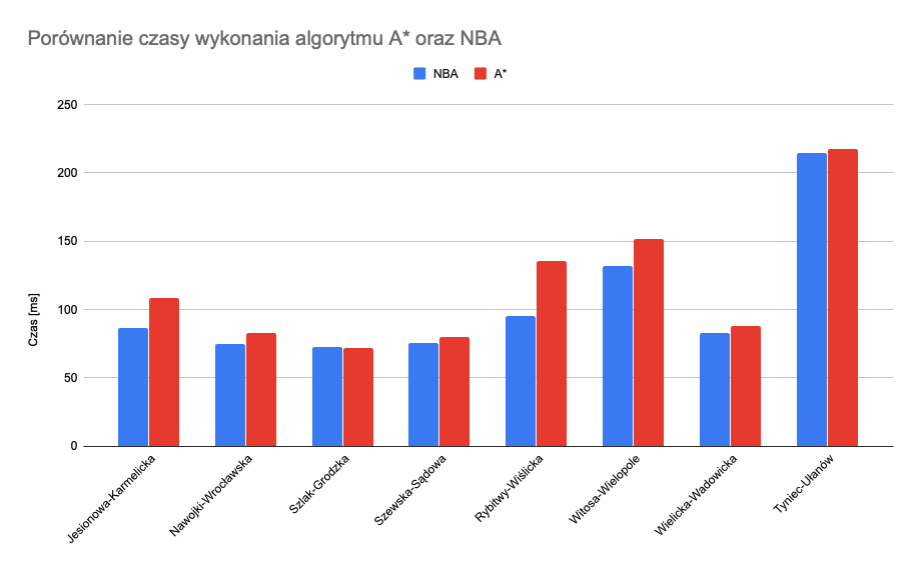
\includegraphics[width=0.7\textwidth]{czas_a_vs_nba}
\caption{Zestawienie czasu wykonania algorytmu A* oraz NBA dla wybranego zestawu danych testowych.}
\end{figure}

Z otrzymanych wyników można odczytać, że algorytm NBA daje możliwość uzyskania nieznacznie mniejszych czasów obliczeń. Same różnice nie są duże, ale znikomym nakładem pozwalają nieznacznie obniżyć wykorzystanie zasobów serwera w przypadku, gdy aplikacja jest używana przez sporą ilość ludzi. Z wykresu można także odczytać nieznaczny trend w kierunku zwiększenia różnic czasów wykonania algorytmu w przypadku, gdy trasy są dłuższe. Jest to spowodowane faktem, że zasoby czasowe potrzebne na alokację oraz rozpoczęcie procedury przeszukiwania grafu z obydwu stron mogą być skompensowane przez rzeczywisty zysk uzyskany przez samą procedurę przeszukiwania. Czas obliczeń dla tras o długości 800-2000m jest w przypadku obydwu algorytmów prawie taki sam.

\subsection{Przeprowadzenie testu użycia procesora dla aplikacji serwerowej w zależności od zastosowania algorytmu A* lub NBA}

Korzystając z wiedzy odnośnie czasu wykonywania oraz jakości analizowanych algorytmów, zostały wybrane dwa z nich, które gwarantują wyszukanie optymalnej ścieżki w grafie. Nie tylko bliskiej rozwiązaniu optymalnemu, jak w przypadku A* zachłannego. Wybrane algorytmy gwarantują czas wykonywania umożliwiający swobodne działanie aplikacji w środowisku produkcyjnym. W tym kroku został także odrzucony algorytm Dijkstra, jako że czas jego wykonania uniemożliwiał swobodne korzystanie z aplikacji przez użytkowników. Dla wybranych algorytmów, A* i NBA, zostały przeprowadzone testy które miały na celu pomiar użycia mikroprocesora podczas wykonywanych przez komputer obliczeń. Do pomiaru aktualnego użycia procesora została użyta wbudowana aplikacja ps, wyniki zostały przedstawione na poniższych wykresach.

\begin{figure}[H]
\centering
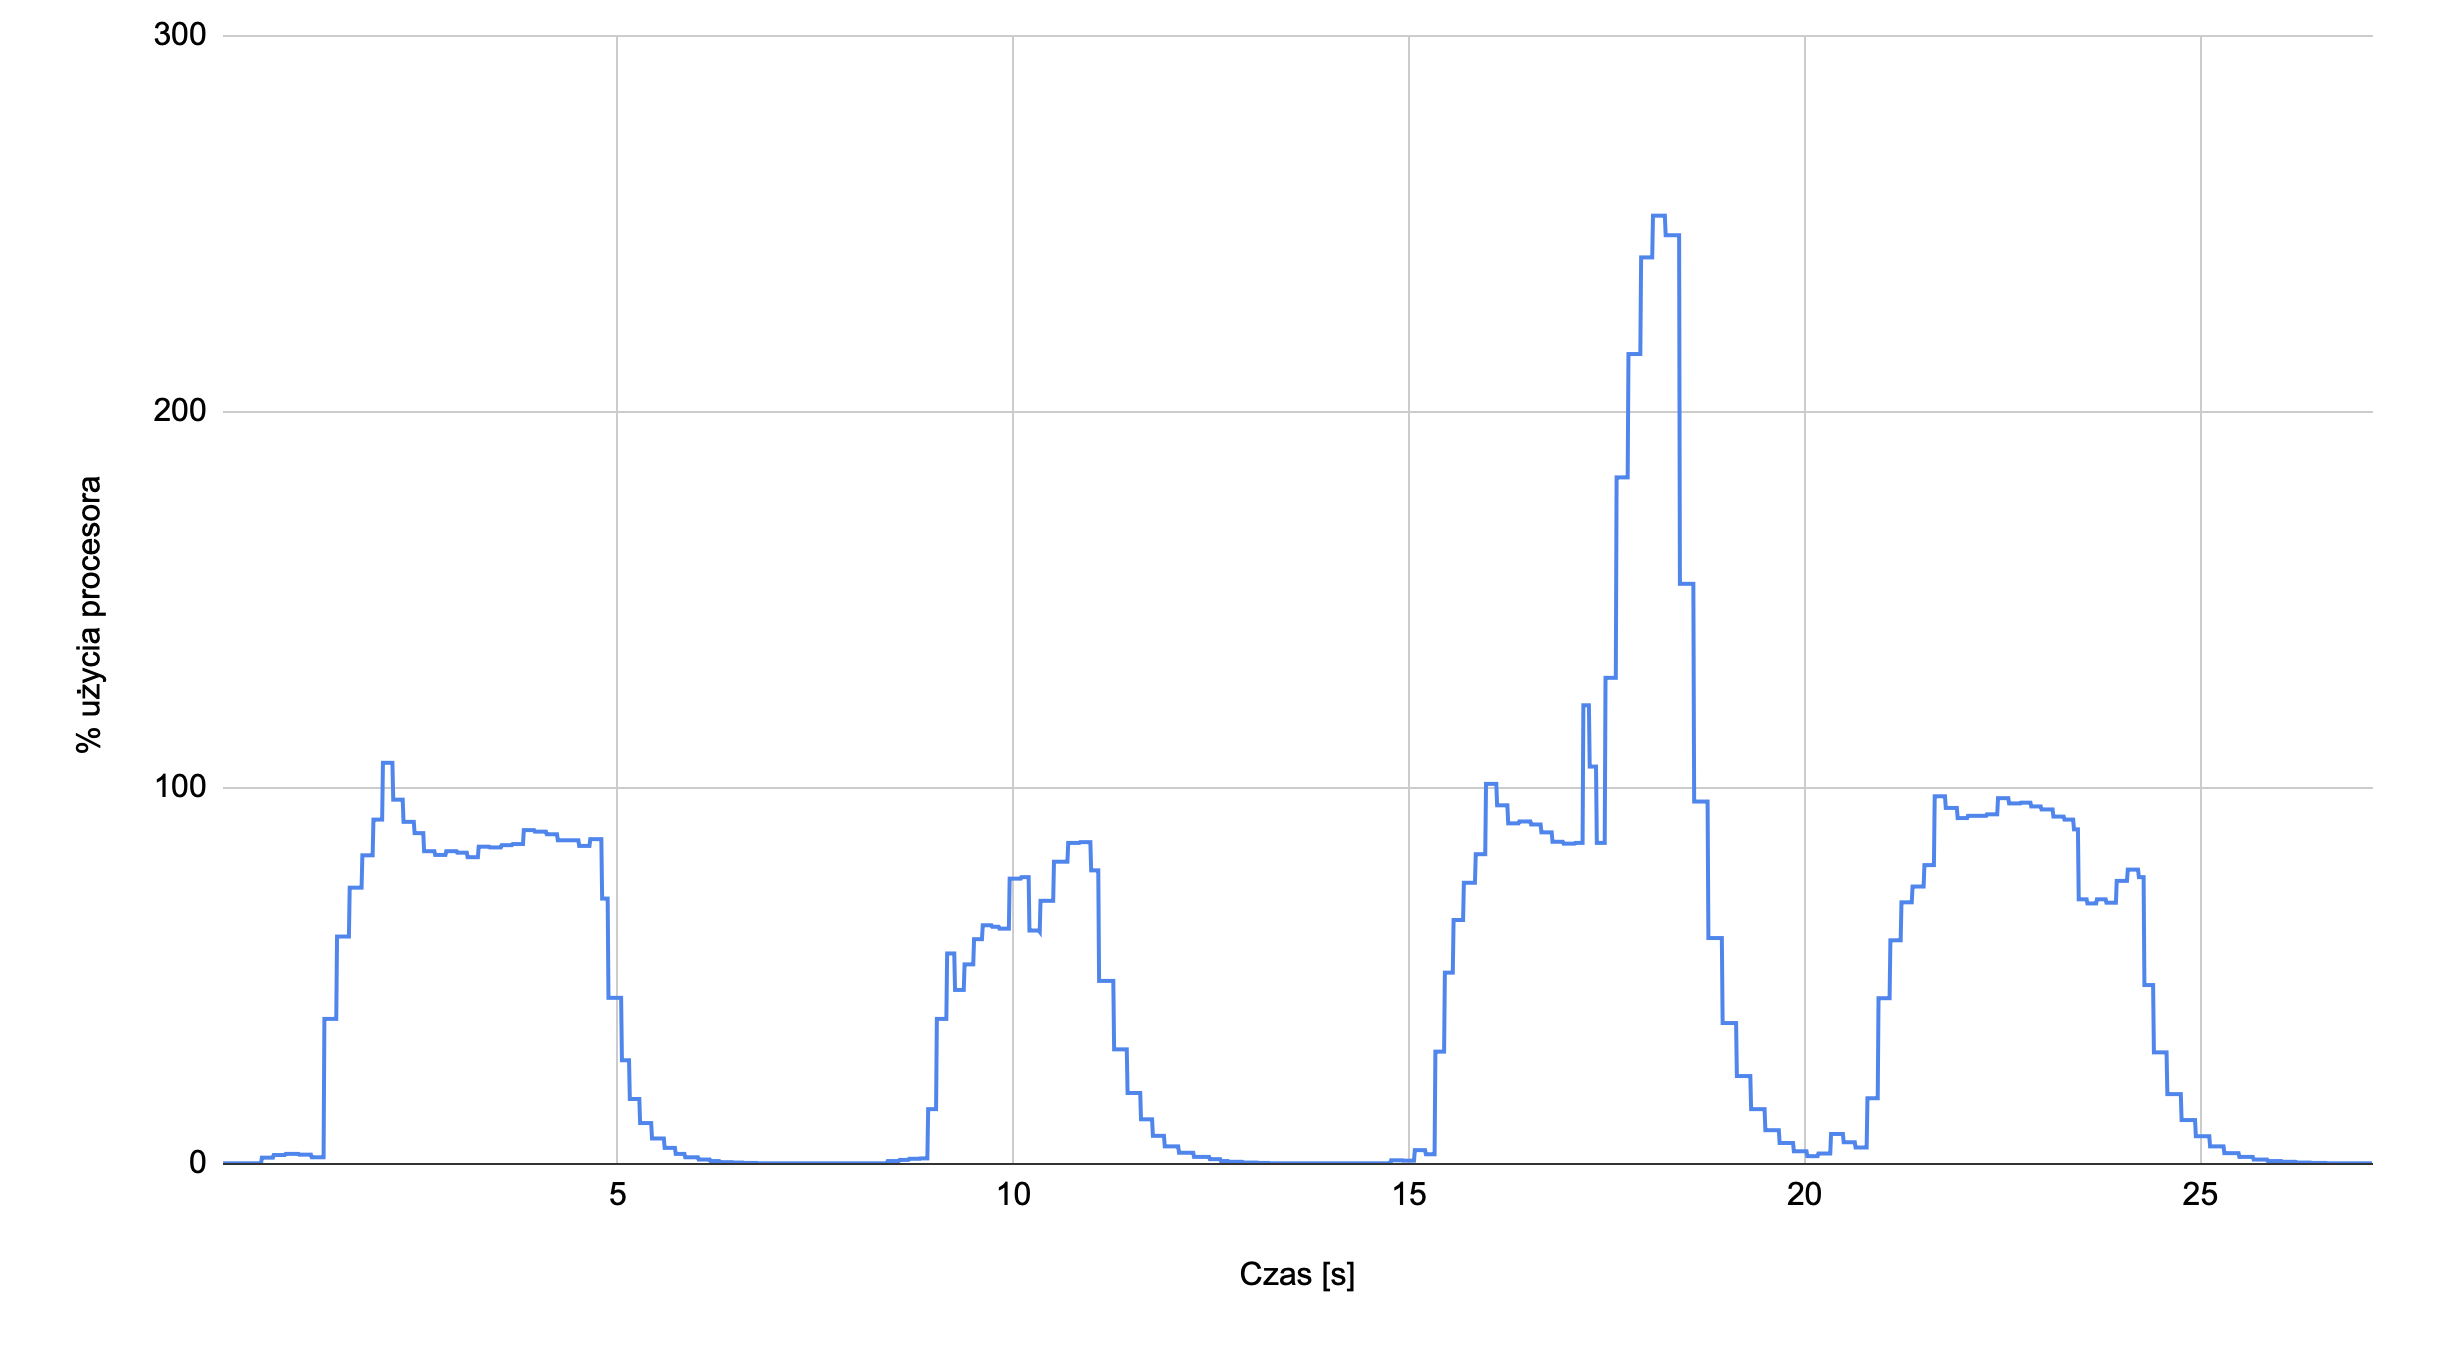
\includegraphics[width=0.7\textwidth]{a_star_cpu}
\caption{Wykres procentowego użycia procesora przy wykonywaniu algorytmu A*.}
\end{figure}

\begin{figure}[H]
\centering
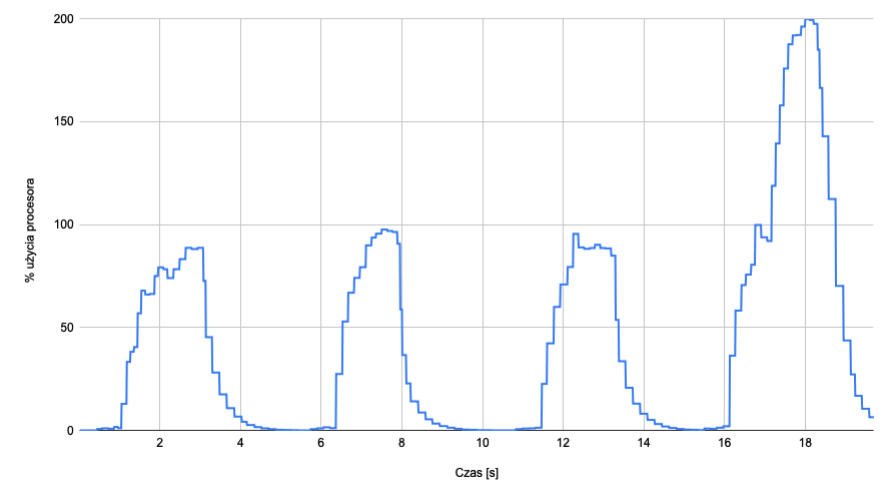
\includegraphics[width=0.7\textwidth]{nba_cpu}
\caption{Wykres procentowego użycia procesora przy wykonywaniu algorytmu NBA.}
\end{figure}

Na przedstawionych wykresach każda ze szpilek oznacza pojedyncze wykonanie zapytania do serwera, więc także obliczenie algorytmu. Test ma na celu sprawdzenie czy obydwa użyte algorytmu podczas swojego działania używają maksymalnych zasobów mikroprocesora maszyny na której są włączane. Z wykresów można odczytać że algorytmy wykazują podobne użycie procesora. Szpilki wychodzące powyżej dwustu lub nawet trzystu procent są związane z dodatkowymi procesami włączanymi przez środowisko Node podczas wykonywania zapytań a wyjście powyżej stu procent użycia procesora oznacza użycie wielu rdzeni jednocześnie.

\section{Porównanie wyników w stosunku do tras wyznaczonych przez Google Maps}

W celu przedstawienia rzeczywistego kontekstu dla przeprowadzanych pomiarów, w ostatnim punkcie porównania dokonano analizy tras wyznaczanych przez stworzoną aplikację w stosunku do tych wyznaczanych przez najbardziej popularną wyszukiwarkę tras zarówno samochodowych, rowerowych, jak i pieszych oferowaną przez Google Maps. Na poniższym wykresie przedstawiono zestawienie długości wyznaczonych tras w zależności od wybranej opcji trasy, najkrótszą lub najlepszą, z odpowiadającą temu trasą Google.

\begin{figure}[H]
\centering
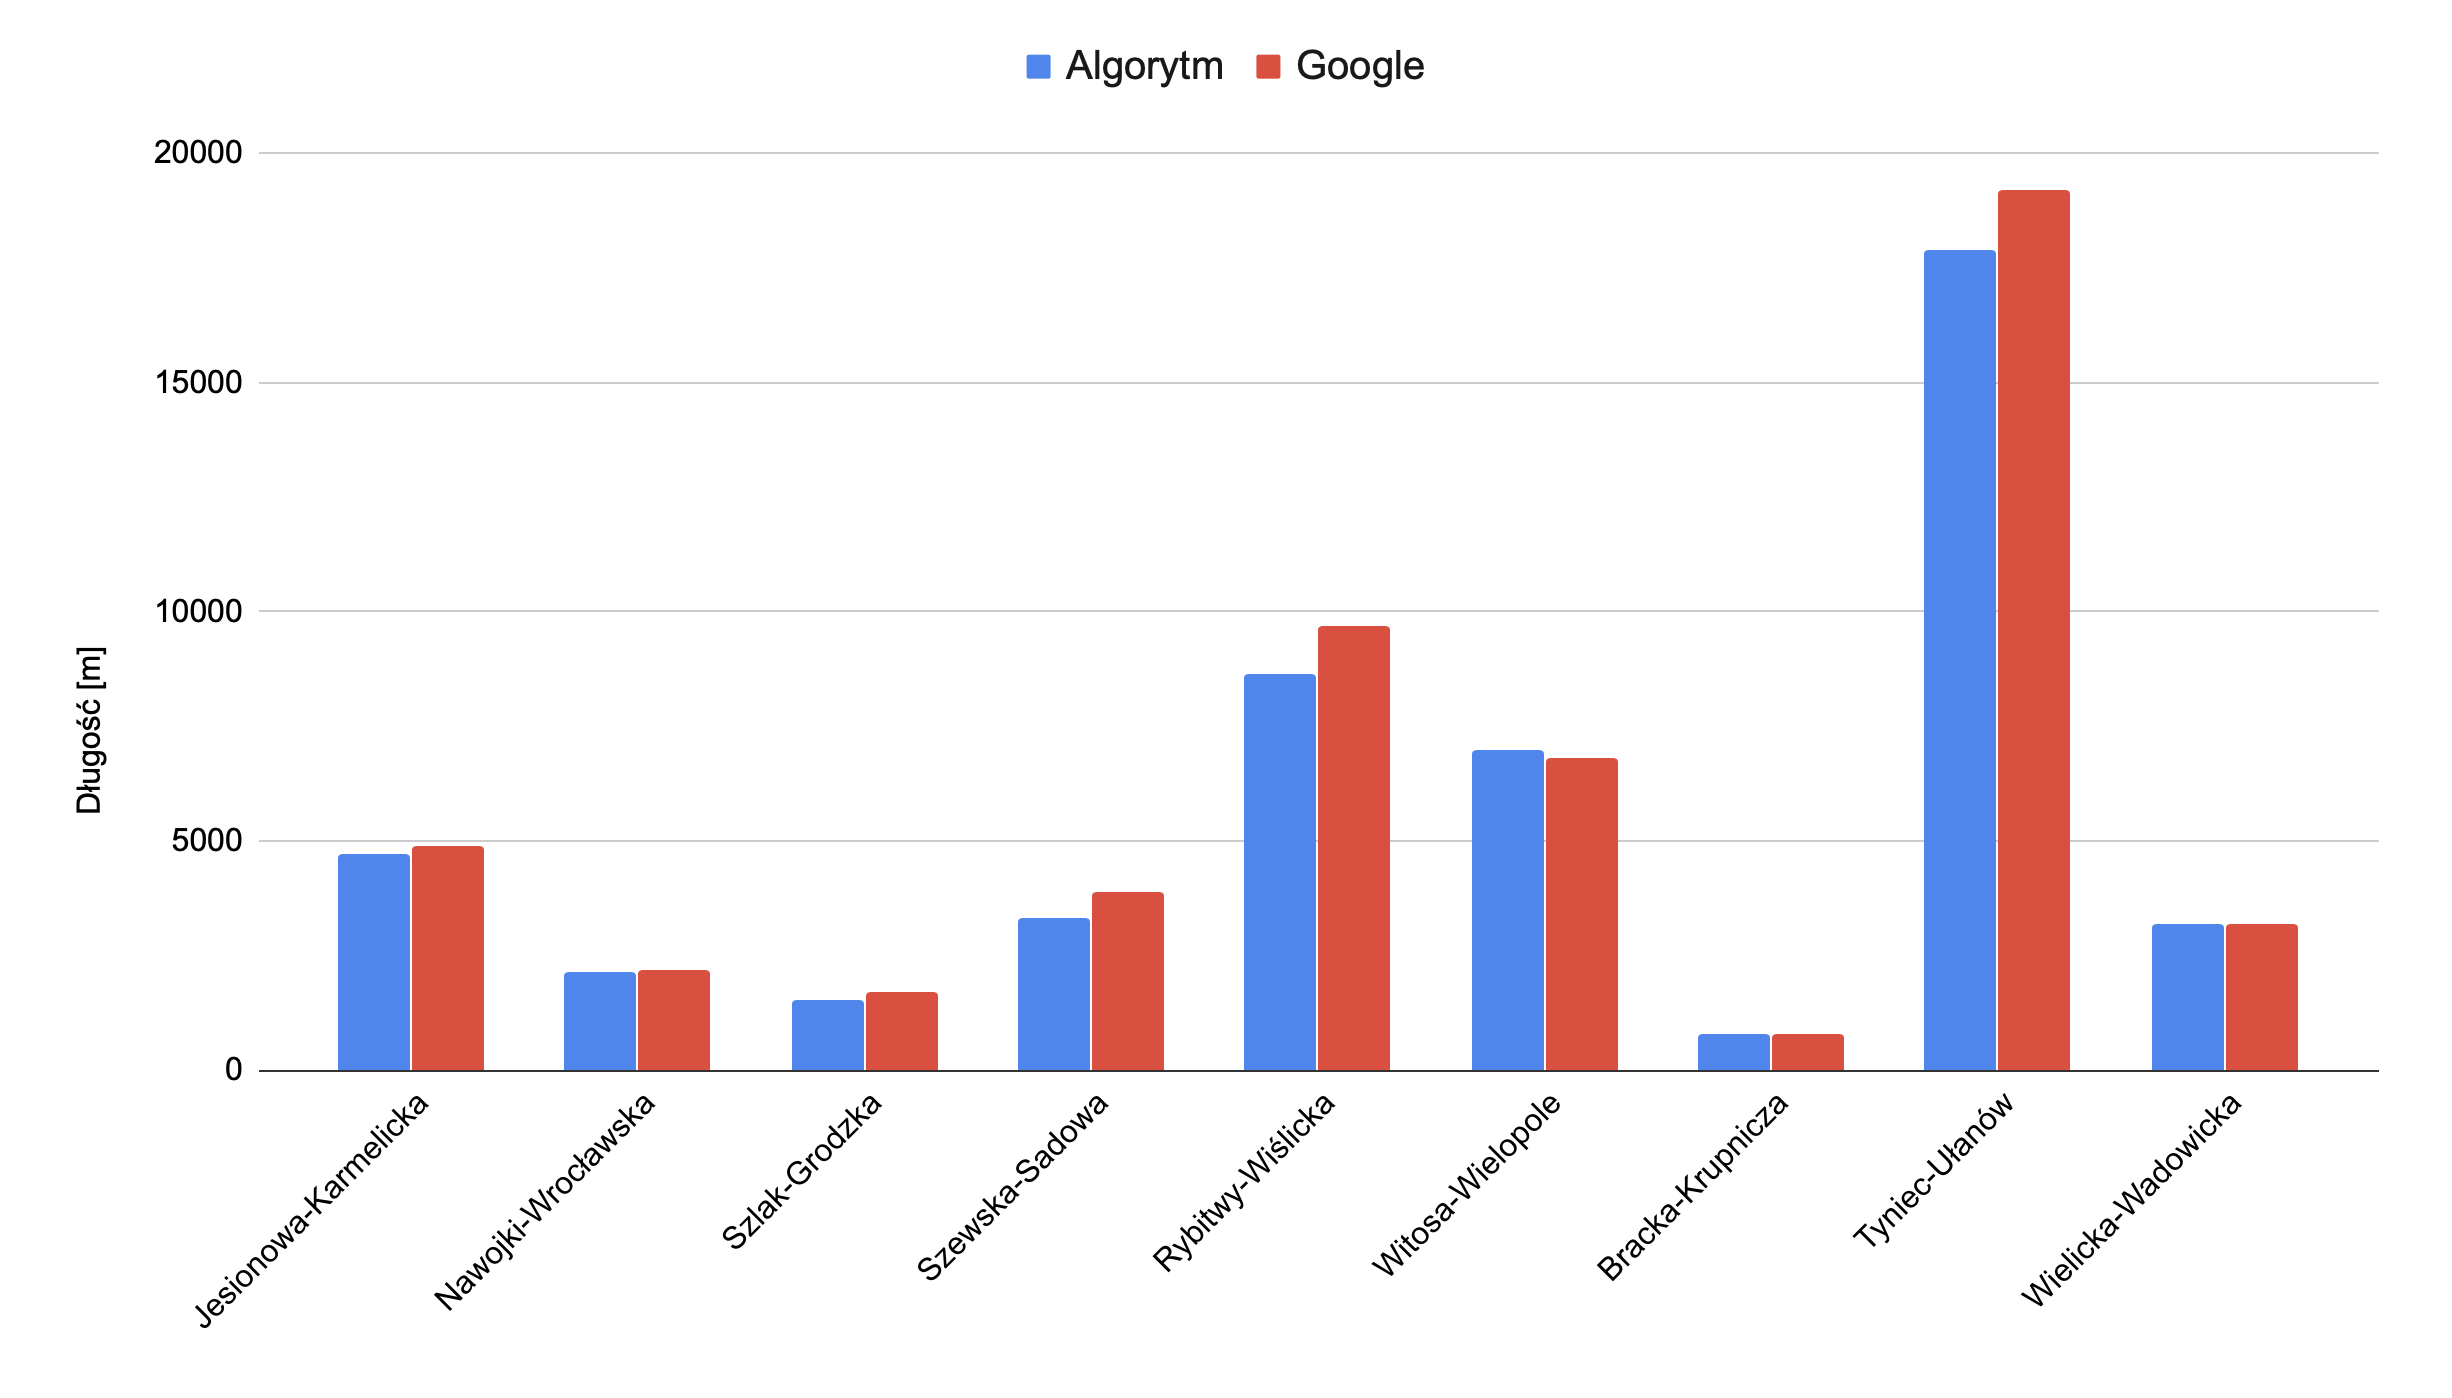
\includegraphics[width=0.7\textwidth]{google_vs_algo_najkrotsza}
\caption{Porównanie długości tras wyznaczonych przez aplikację oraz Google Map przy wyborze najkrótszej trasy.}
\end{figure}

\begin{figure}[H]
\centering
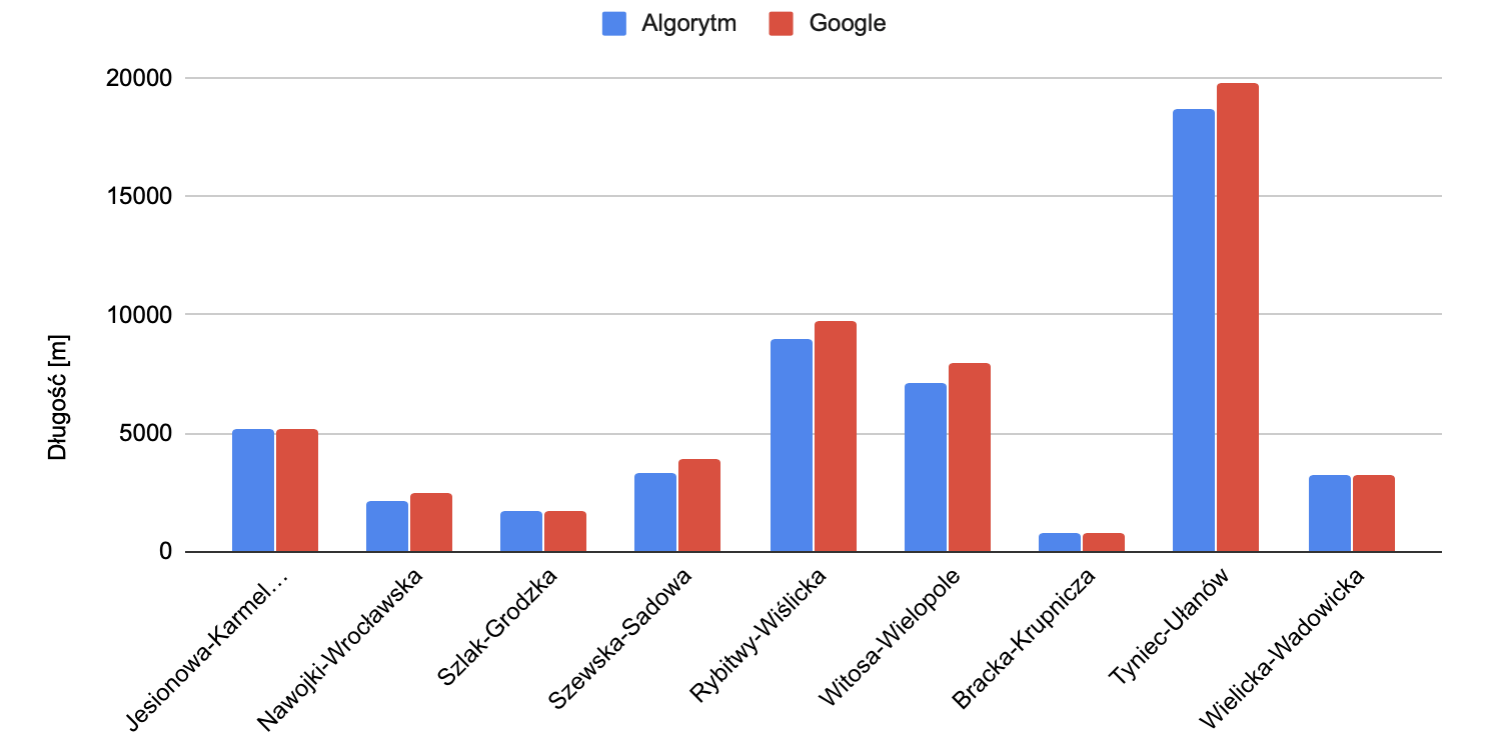
\includegraphics[width=0.7\textwidth]{google_vs_algo_najlepsza}
\caption{Porównanie długości tras wyznaczonych przez aplikację oraz Google Map przy wyborze najlepszej trasy.}
\end{figure}

Z powyższych porównań można odczytać, że w większości przypadków, zaproponowany algorytm wyznaczył trasy krótsze niż wyszukiwarka Google. W przypadku nieznacznych różnic może to być spowodowane przez różne poprowadzenie punktów na mapie składających się na drogi, można jednak znaleźć 3 przypadki, w których trasy zostały poprowadzone inaczej i skutkowało to ich skróceniem. Dodatkowym zyskiem podczas korzystania z zaproponowanego rozwiązania jest pewność, że użytkownik zostanie poprowadzony przez drogi dla rowerów lub miejsca umożliwiające swobodne poruszanie się na rowerze. W przypadku map Google trasa wyznaczana jest także po ulicach bez zmniejszonych ograniczeń prędkości. Niestety dostęp do algorytmu wyznaczania tras przez aplikację Google jest zamknięty, nie jesteśmy w stanie bezpośrednio porównać działania obydwu algorytmów, możemy jednak na podstawie obserwacji przewidywać. Różnica w działaniu, działająca na korzyść  rozwiązania będącego przedmiotem tej pracy, jest spowodowana głównie brakiem odpowiednich danych odnośnie dróg typu kontrapas poprowadzonych w przeciwnym kierunku w stosunku do jednokierunkowych ulic dla samochodów.